\section{Technical Approach}
\subsection{Input FSM Specification}
The input minimal FSM can be an arbitrary FSM with the following restrictions:

{\bf (1)} The input FSM must communicate to the outside world through ready/valid ports  

{\bf (2)} The designer cannot use input valid or output ready signals as inputs to any part of their circuit

{\bf (3)} Any functional units that may take more than one clock cycle to return responses(caches, multipliers, dividers, etc) must be accessed through the Variable Latency Unit Interface discussed below.

\subsubsection{IO Semantics}
When input ready or output valid is driven high by the input FSM, this implicity signals to the tool that the input FSM requires the use of the input or output port on the current state update. Thus, the tool generates logic that examines the input ready or output valid and stalls the pipeline if the corresponding input valid or output ready is not driven high by external modules. The designer should design the input FSM so that input readies and output valids are only driven high when absolutely necessary to avoid unnecessary stalling the automatically multi-threaded and pipelined version of the circuit.

\begin{figure}
	\centering
    \resizebox{\columnwidth}{!}{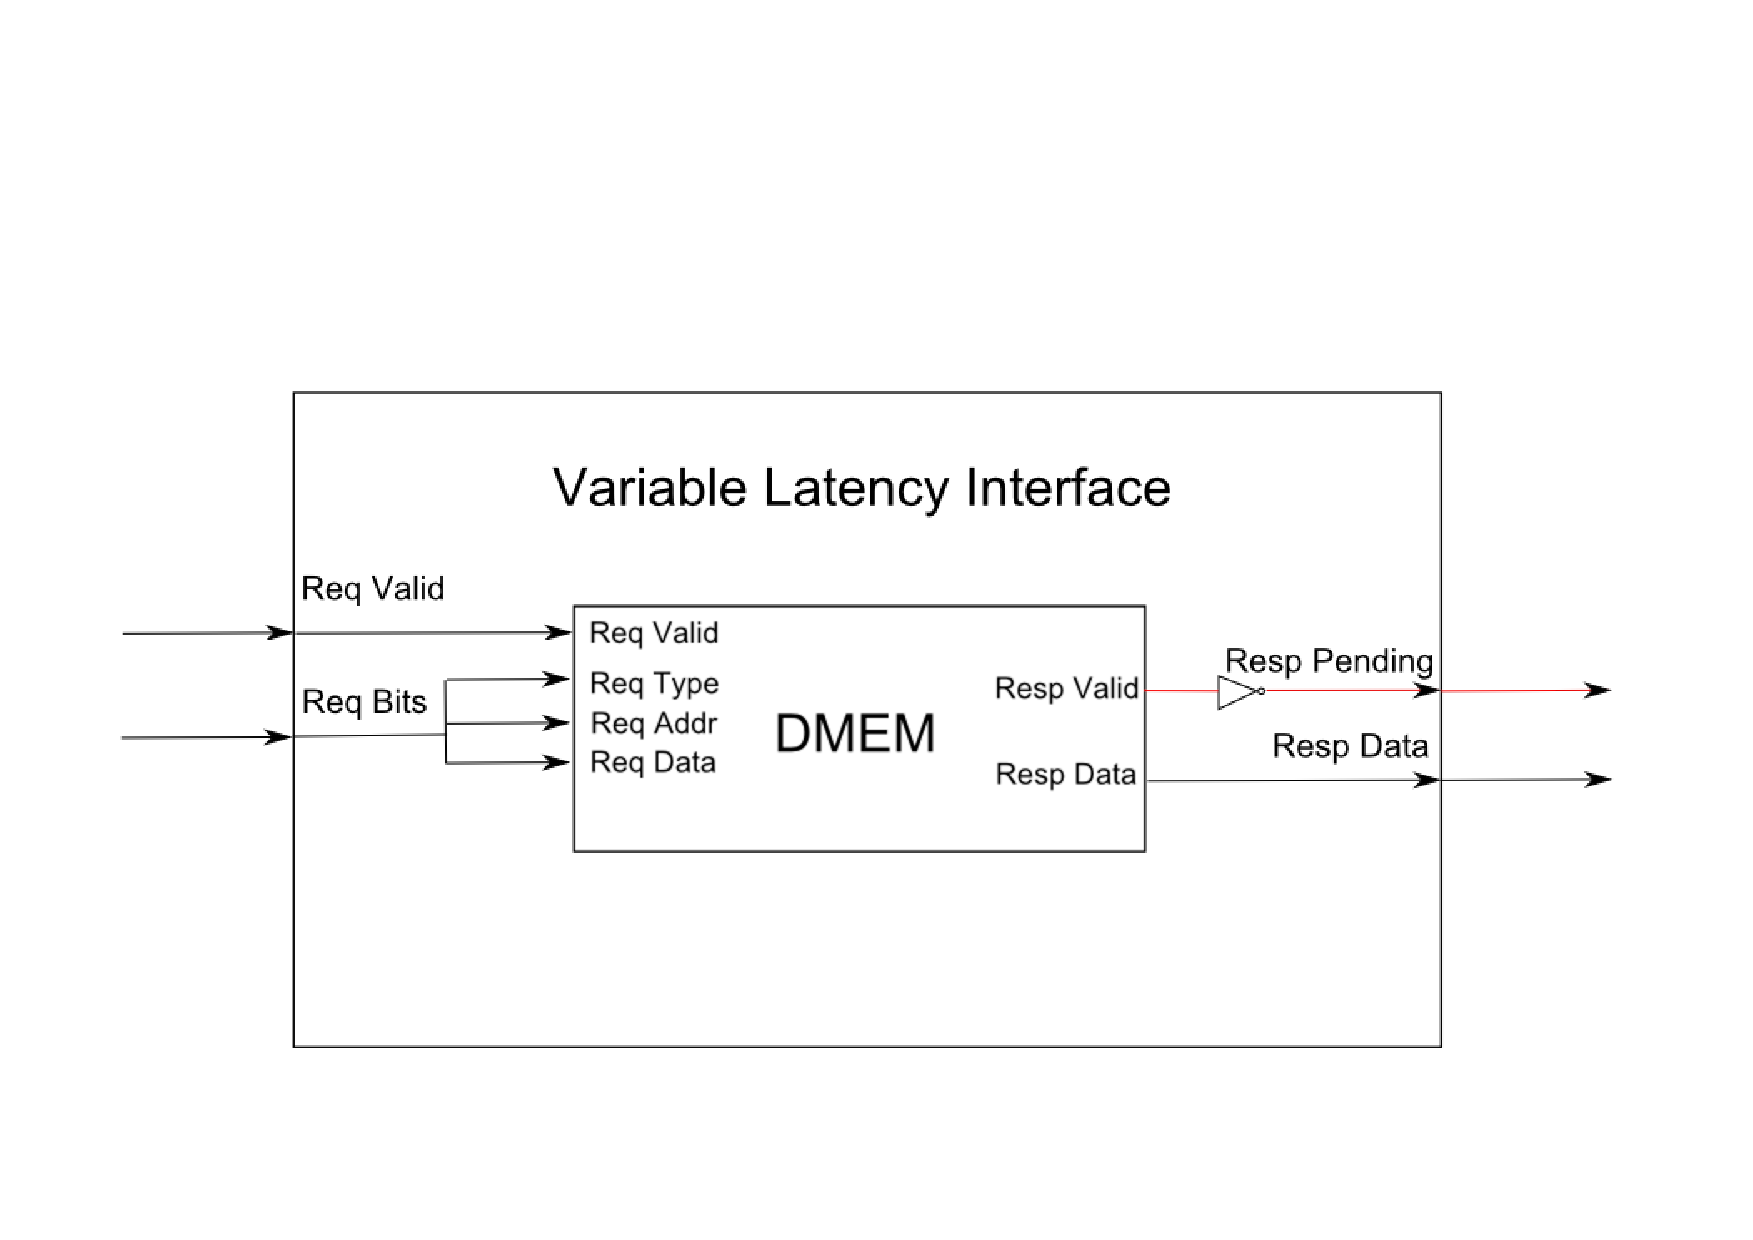
\includegraphics{figures/TransactionalInterface}}
    \caption{{\bf Single Thread View of Variable Latency Unit Interface} Black wire are user facing IO, red wires are tool facing IO}
	\label{fig:VarLatIO}
\end{figure}

\subsubsection{Variable Latency Unit Interface}
In order to accomodate caches and long latency arithmetic units in the minimal FSM specification that is not allowed to have any optimization or control logic implemented, the tool provides the Variable Latency Unit Interface. The designer should access any caches or long latency arithmetic units through a Variable Latency Unit Interface and treat that Variable Latency Unit Interface like a piece of combinational logic in the input FSM specification. IE the designer should not use the Resp Pending port of the Variable Latency Unit Interface to drive any part of their circuit and should pretend that the Variable Latency Unit Interface always gives a valid response immediately. The tool will automatically generate control logic that deals with the Variable Latency Unit Interface not immediately outputting a valid response.

When the tool does the multithreading transformation, each Variable Latency Unit Interface in the input minimal FSM is replicated n times, where n is the number of threads. It is up to the designer to create glue logic that deals the copies of the Variable Latency Unit Interfaces in a top level module that instantiates the automatically multi-threaded module. The designer can instantiate n copies of the functional unit, one for each Variable Latency Unit Interface, or can create additional logic that multiplexes all copies of the Variable Latency Unit Interface onto a single functional unit.

\subsection{Minimal FSM Transformation}
Given an input minimal FSM, the tool analyzes the node graph that represents the FSM and modifies the node graph to generate a multi-threaded, pipelined design that is functionally equivalent to n copies of the input FSM, where n is the number of threads.

In order to make analysis of the input FSM easier, the tool breaks up the state elements into read and write ports. This results in an acyclic node graph in which data flows from the state element read ports and the input data ports to the state element write ports and output data   ports. For the figures in this section, state elements are draw as separate "r" and "w" pieces.

Figure \ref{fig:initialFSM}. and Figure \ref{fig:finalFSM}. show an example initial input minimal FSM and the final multi-threaded, pipelined FSM after the transformation. The rest of this section describes the transformations that are performed.

\begin{figure}
	\centering
    \resizebox{\columnwidth}{!}{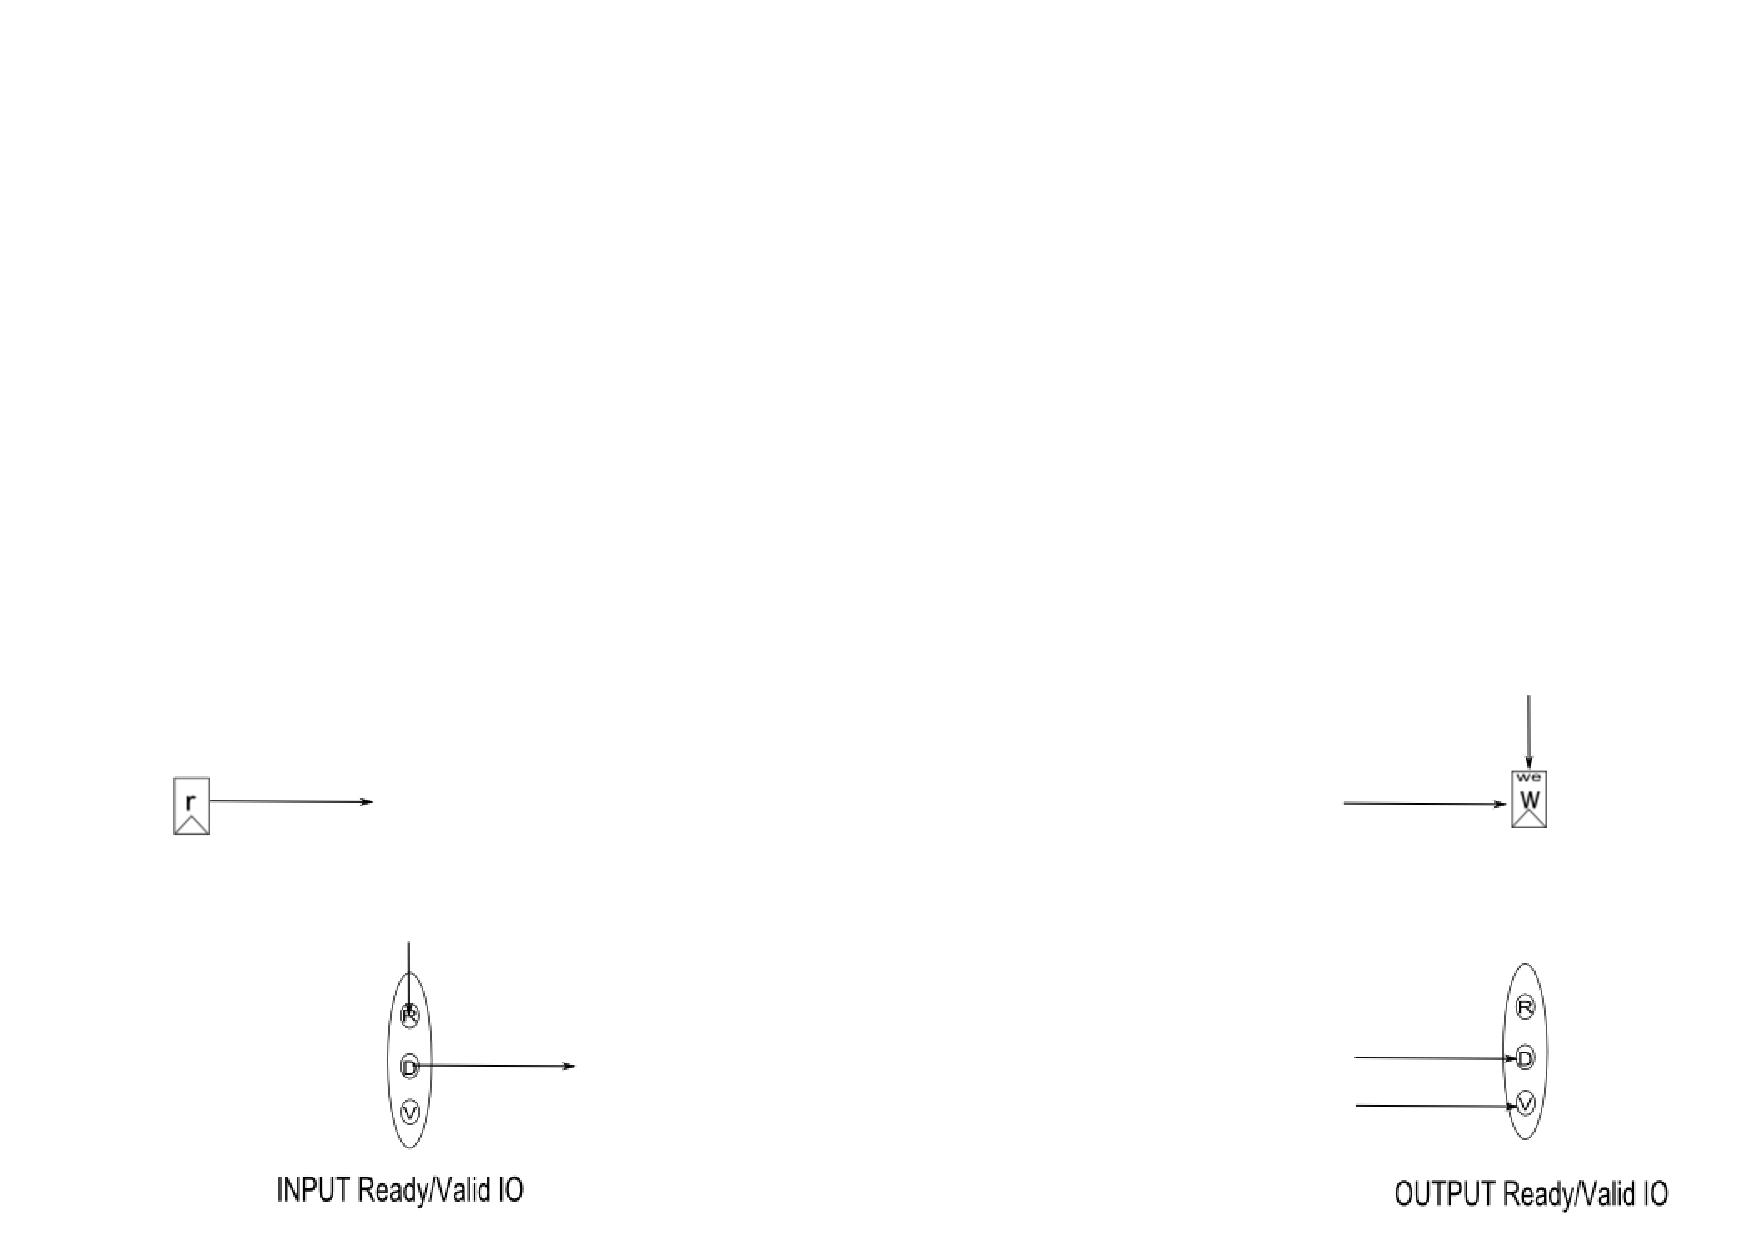
\includegraphics{figures/initialFSM}}
    \caption{{\bf Input Minimal FSM} The input FSM consists of one register, one input port, and one output port. The register is split up into read and write ports. The combinational logic is not shown.}
	\label{fig:initialFSM}
\end{figure}

\begin{figure}
	\centering
    \resizebox{\columnwidth}{!}{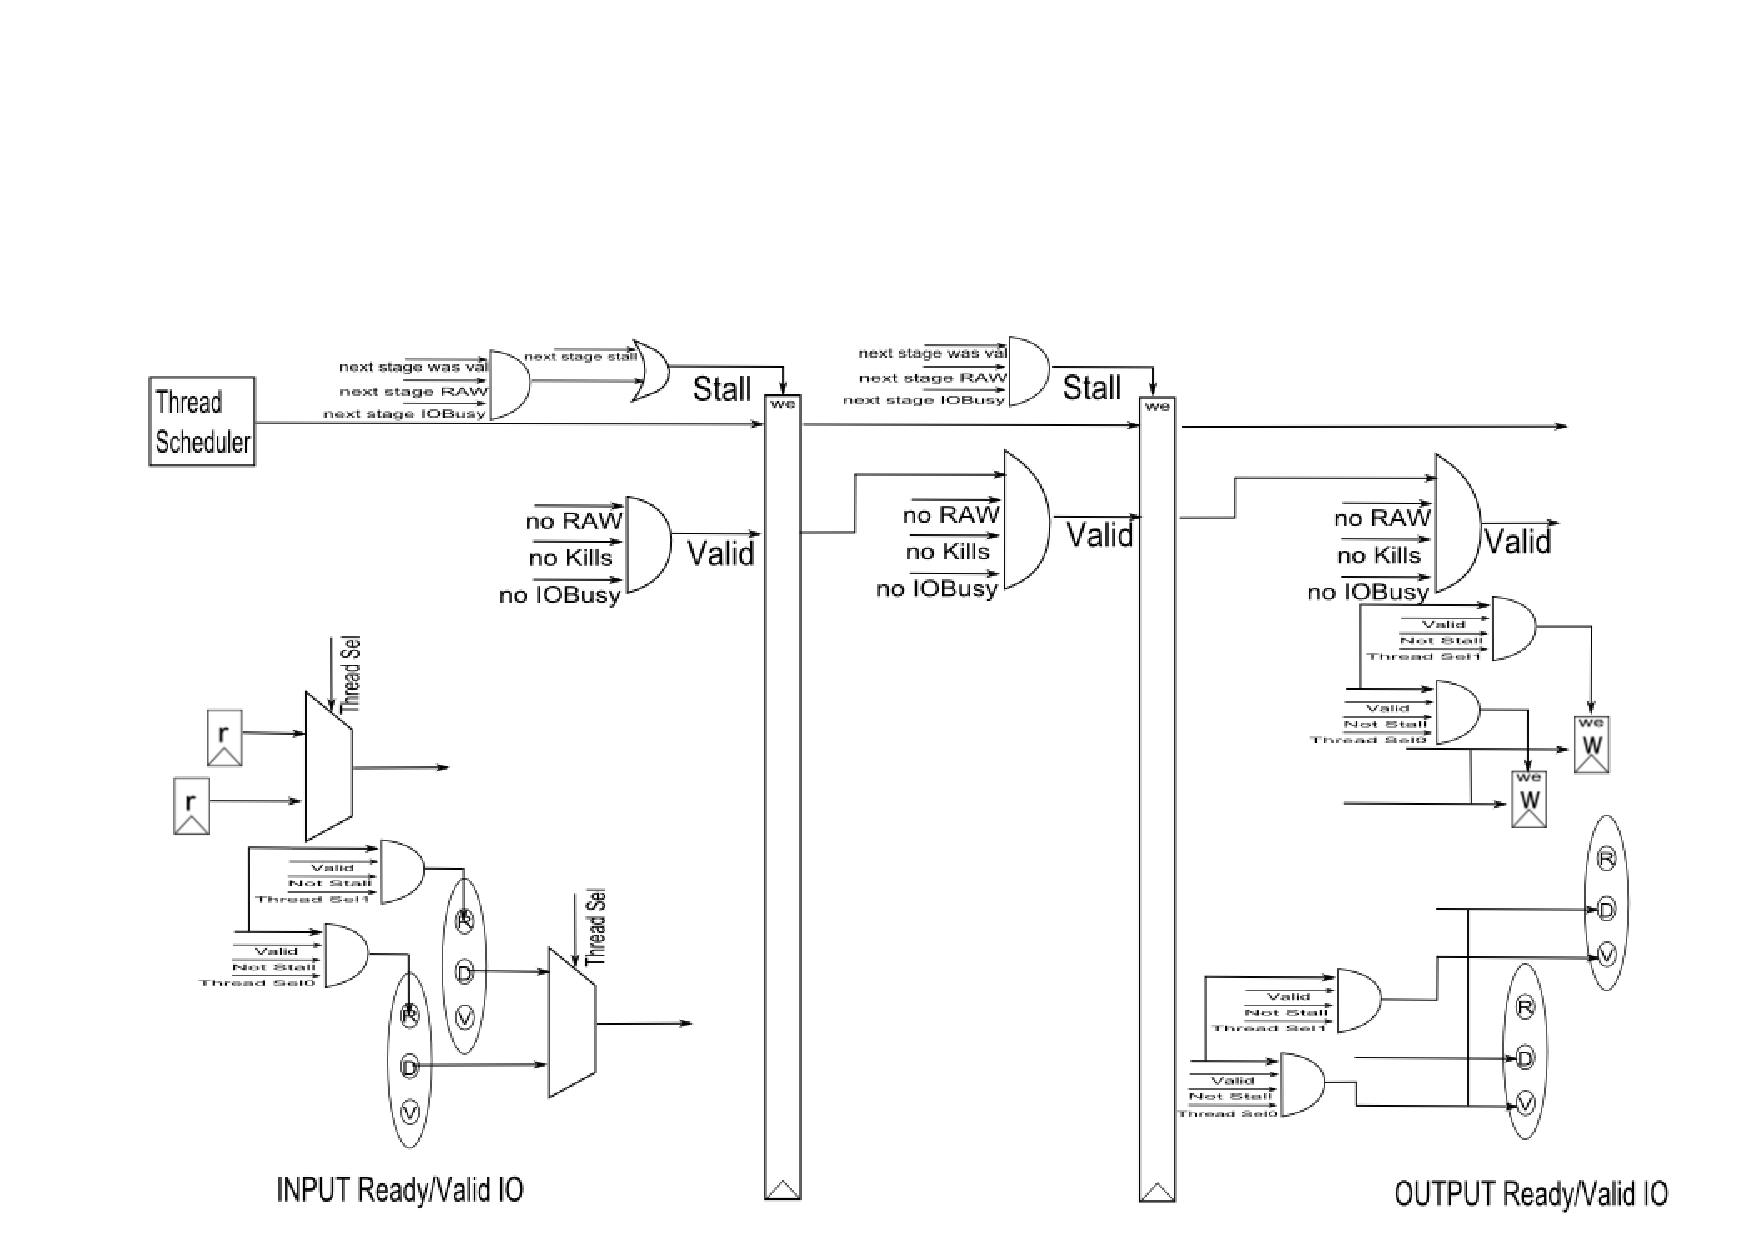
\includegraphics{figures/finalFSM}}
    \caption{{\bf Final Multi-threaded, Pipelined FSM} This is a 2 thread, 3 stage version of the input FSM with all of the generated control logic shown. The cominational logic is not shown.}
	\label{fig:finalFSM}
\end{figure}

\subsection{State and IO replication}
\label{sec:replication}
Given a user specification of n threads, the tool first replicates the IO ports the state elements n times. The input ready signals, output data signals, and the output valid signals of the replicated IO elements are driven by the corresponding original IO port signals. The state element write data signals, and state element write enable signals of the replicated state elements are drive by the corresponding original state element write signals. 

A mux is placed infront of the input data signals and all consumers of the original input data signal is now driven by this mux. Similarly, a mux is placed infront of the replicated state element read data signals and all consumers of the original read data signal is now drive by this mux.

\subsection{Pipeline Register Insertion}
Given a user specification of m pipeline stages, the tool inserts m - 1 pipeline registers into the design. The tool automatically finds a legal placement of the registers that satisfy the following rules:

{\bf (1)} Every combinational logic node has all input signal with the same stage number.  

{\bf (2)} The stage number of every combinational logic node's output signal is equal to the shared stage number of its input signals.

{\bf (3)} There are two ways to determine the stage number of a node. One way is to trace through the node's inputs to a pipeline register and set the stage number of the node equal to the stage number of that pipeline register. Another way is to trace through the node’s consumers to a pipeline register and set the stage number of the node equal to the stage number of that pipeline register {\tt -}  1. For all nodes in the graph, the stage number of the node obtained through both methods must be the same.

Then the tool automatically optimizes the pipeline register placement with regards to critical path delay by balancing the longest path delays for each pipeline stage. The details of how this is done will not be discussed in the paper as it was part of the previous automatic pipelining project.

\subsection{Control Logic Generation}
The tool then inserts logic that generates thread select and pipeline control signals. 

\subsubsection{IOBusy Signals}
An IO port is considered busy if it belongs to the thread that matches the thread ID signal in the IO port's stage and if the input ready/output valid signal is driven high, which implicitly signals that the data from this port is needed to be consumed/produced, and the input valid/output ready signal is driven low by an outside module, which indicates that the port is not available.

\subsubsection{RAW Hazard Signals}
A read port belonging to thread N, stage X is considered to have a RAW hazard if a pipeline stage Y is valid, has the same thread ID as stage X, and contains a transaction that could write to any write port that belongs to the same state element as the read port.

\subsubsection{Kill Signals}
A stage is killed if a Variable Latency Unit IO in that stage drives RespPending high and the thread ID signal of the stage equals the thread that Variable Latency Unit IO belongs in.

\subsubsection{ThreadID signals}
The tool pipelines the thread ID signal generated by the thread scheduler so that it is available for each pipeline stage. The thread ID signal in each pipeline stage is wired into the muxes generated in \ref{sec:replication}. The input ready signals, output valid signals, Variable Latency Unit Interface Req Valid signals, and state element write enable signal are masked with the thread ID signal for the pipeline stage they belong in.

\subsubsection{Valid Signals}
The tool generates a valid signal for each pipeline stage. Each pipeline stage is currently valid if the previous pipline stage was valid on the last clock cycle, no state element read ports in this pipeline stage has a RAW hazard, no IO port in this stage is busy, and there are no kill signals triggered in this stage. The input ready signals, output valid signals, Variable Latency Unit Interface Req Valid signals, and state element write enable signal are masked with the valid signal for the pipeline stage they belong in.

\subsubsection{Stall Signals}
The tool generates a stall signal for each pipeline stage. When a pipeline stage is stalled, the contents of that pipeline stage does not progress into the next pipeline stage. The boolean equation for stage X's stall signal = stage X + 1 is stalled OR (stage X was valid last cycle AND (a read port in stage X+1 has a RAW hazard OR a IO port in stage X+1 is busy)). The input ready signals, output valid signals, Variable Latency Unit Interface Req Valid signals, and state element write enable signal are masked with the valid signal for the pipeline stage they belong in. 
